In this chapter are collected interpretations of the results obtained in the Feature Selection and the models' performance. All other tests not included in this chapter are available in the appendix \ref{chap:appendix}.
\\
\section{Feature Selection Results}
In this section the results obtained for each target variable selected are explained in relation to the:
\begin{itemize}
    \item votes received through Borda Count algorithm;
    \item positive or negative correlation assumed in the filter methods;
    \item confirmation in literature where a given correlation occurred; 
\end{itemize}
Similarities between the tests run for each target variable are visible for many factors that influence both particulate matter and ammonia.\\
This can be observed by the similarity of both positive and negative correlations from indexes obtained by filter methods. \\
The results of the Pearson index, a filter method used during the FS, are shown in figure \ref{fig:pearson_general}. 
\begin{figure}[H]
\centering
\subfloat[pm25\_st as target variable.]{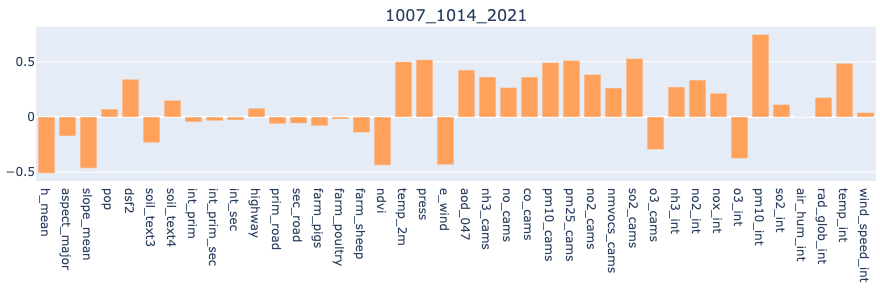
\includegraphics[scale =0.45]{images/tests/pm25pearson_october_0_01_mountains.png}}\\
\subfloat[nh3\_st as target variable.]{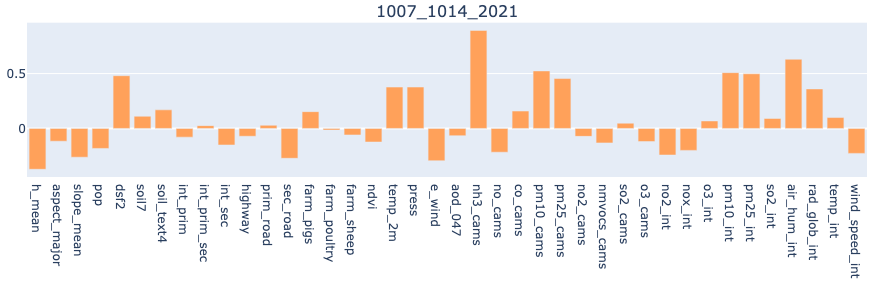
\includegraphics[scale =0.45]{images/tests/nh3_pearson_october_0_01_mountains.png}}
\caption{Pearson index results obtained in the period between 7-14 October with 1km resolution including mountains.}
\label{fig:pearson_general}
\end{figure}
The two bar plots attached aim to compare the scores obtained in the same period by the 2 target variables chosen in my tests in the October period.
One similarity between them is the influence of meteorological and morphological parameters.
By figure, it appears that DTM average elevation and slope ('h\_mean' and 'slope\_mean' respectively) are correlated in the same way in the test of both target variables since air pollution affects more urban than mountain areas.\\
Pollutants are negatively correlated to wind speed ('e\_wind'), since their concentration tends to turn down with it.\\ 
Indeed, the wind is a marker for the horizontal transport of air pollutants. Pressure also contributes to them ('press'), since it causes stable atmospheric conditions that make pollutants harder to be disseminated.
\par
In the test run the findings did not discover consistent differences if Alpes and Prealpes zones are included or not.\\
The only slight diversity found is about the votes obtained by pollutant and vegetation variables, which tend to be generally higher if mountain zones are excluded.
\subsection{PM2.5 as target variable}
Fine particulate matter (PM2.5) is one of the most common air pollutants in our environment. 
It comes primarily from transport vehicles (such as cars, trucks and buses), industry, burning of fuels and household activities. \\
During the 5 periods, it has been shown that PM2.5, as the other pollutants, changes over time. Air pollution changes accordingly to the type of climate and atmospheric conditions.\\
Below are attached the table \ref{tab:statspm25} and the figure \ref{fig:graphstatspm2.5} that show PM2.5 variation in the 5 periods chosen in this case study.
\begin{table}[H]
\centering
\begin{tabular}{lrrrrr}
\toprule
 Statistic &  24/03-31/03 &  18/04-25/04 &  17/07-24/07 &  3/09-10/09 &  7/10-14/10 \\
\midrule
  Mean  &        30.217  &         18.203  &         12.974 &       15.450 &       14.878 \\
Median  &        27.938 &        17.938 &        13.063 &       14.75 &       15.281 \\
 Standard deviation &        3.772 &        3.462 &        1.831 &       4.000 &       3.166 \\
  Min value &        20.0  &        11.875 &        9.5 &        8.625 &       9.0 \\
  Max value &        42.0 &        25.714 &        17.375 &        27.875 &       19.625 \\
\bottomrule
\end{tabular}
\caption{Summmary statistics (measured in $\mu$g/m\textsuperscript{3}) of the PM2.5 provided by ARPA with 10 km resolution.}
\label{tab:statspm25}
\end{table}
\begin{figure}[H]
    \centering
    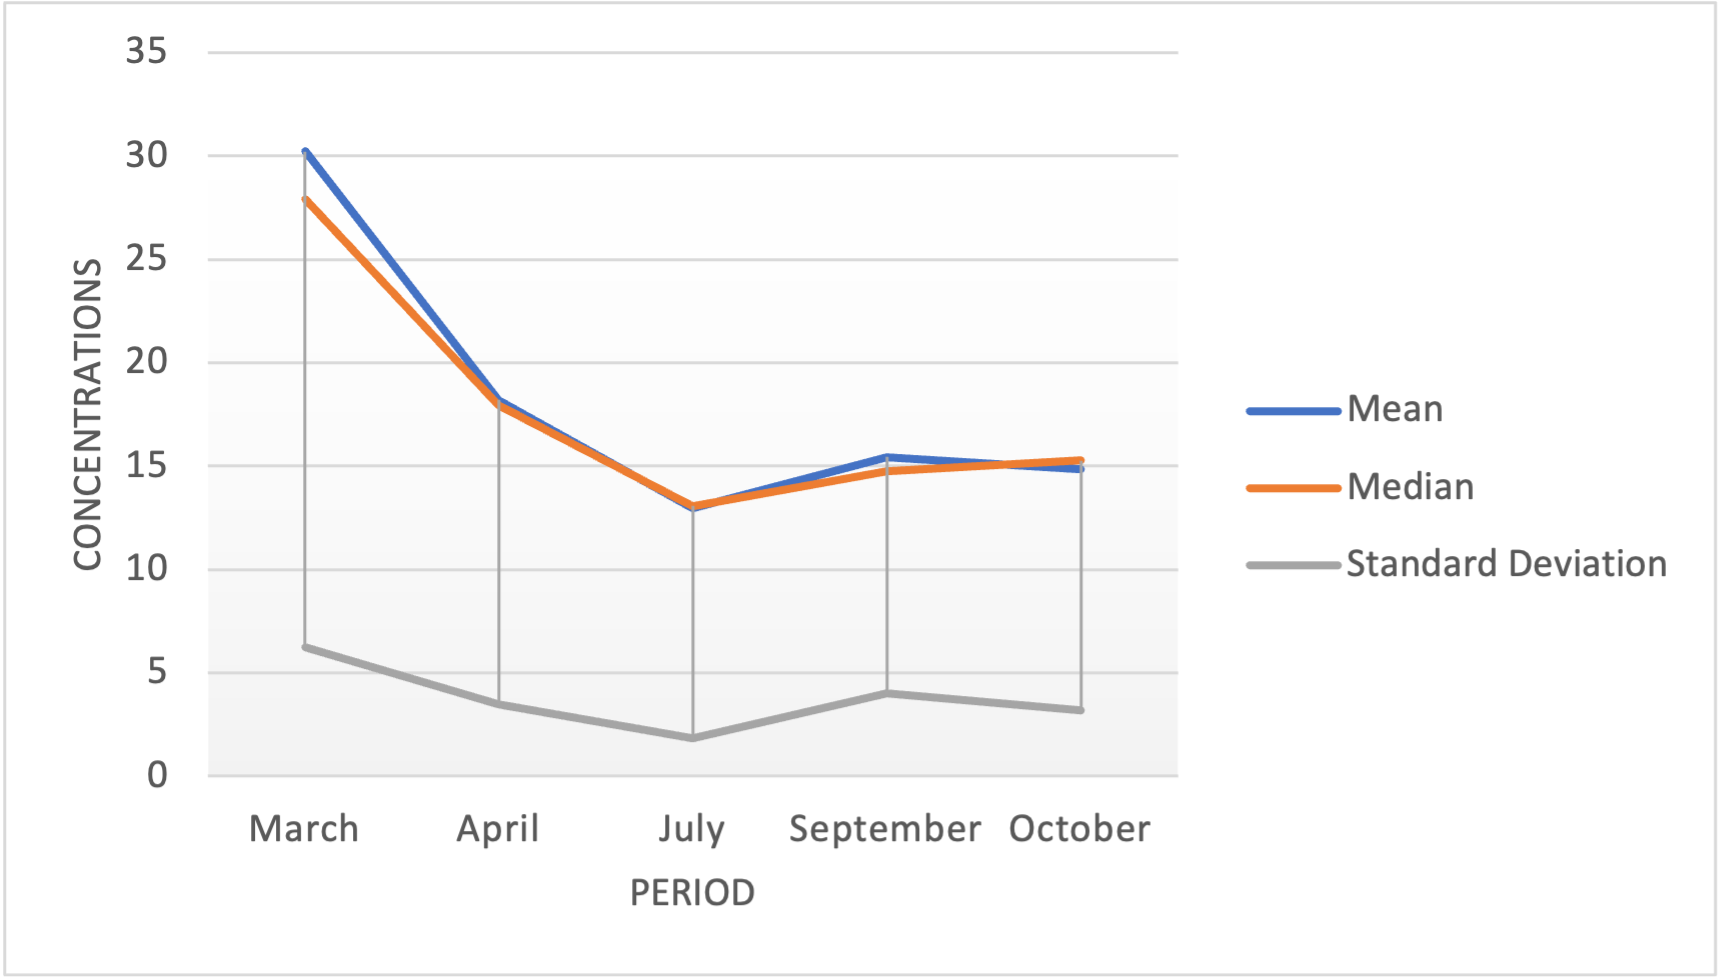
\includegraphics[scale=0.8]{images/pm25_values.png}
    \caption{Graphical representation of PM2.5 variation over the 5 periods, in relation of its mean, median and standard deviation (measured in $\mu$g/m\textsuperscript{3}).}
    \label{fig:graphstatspm2.5}
\end{figure}
In this subsection I comment the results obtained by FS of the figure \ref{fig:a}.
Air pollution analysis can confirm the presence of a high amount in the winter and heating season and a low quantity in the summer months \cite{cichowicz2017dispersion}. This is not applied to the ozone ('o3\_int' and 'o3\_cams'), which should be, on the contrary, higher during summer due to a combination of heat and sunlight which reacts with nitrogen oxides (NOx) and volatile organic compounds.\\
Indeed, ozone receives in the results many votes for its negative correlation (the highest in the summer period), because is inversely related to PM2.5.\\
By the bar plots attached in the figure \ref{fig:fs_pm25}, it is clear that most of the pollutants have a strong or moderate correlation with PM2.5. \\
In particular, PM10 provided by ARPA and CAMS, in the various test executed is one of the most correlated pollutants. Indeed, 'pm10\_int' and 'pm10\_cams' have always had a high number of votes.
A strong positive correlation between PM2.5 and PM10 is also demonstrated in the literature \cite{zhou2016concentrations}.
Another variable which received a strong number of votes is the PM2.5 modelled by CAMS ('pm25\_cams'). \\
Both variables measure the same pollution phenomena.
This finding makes us understand how both variables are correlated even if measurements were performed in 2 different way. PM2.5 from ARPA consists of measurements provided by fixed-ground sensors.\\
Instead, the PM2.5 from CAMS is provided by a global monitoring model, resulting from an ensemble median analysis of other models.
Indeed, the correlation coefficient between them is close to 1 in all tests executed.\\
It is visible a correlation with nitrogen dioxide('no2\_int'), a strong greenhouse gas which is related, as particulate matter, to biomass burning, industrial processes, households and road transport \cite{zellner2000john} \cite{maranzano2022air}.\\
There is also a clear correlation with nitrogen oxides ('nox\_int'), nitrogen monoxide ('no\_int') and carbon monoxide ('co\_int', 'co\_cams, 'co\_s5p'). This could be explained by the fact that these pollutants contribute as a secondary pollutant to PM2.5 formation \cite{xie2015spatiotemporal}.
\par
Observing the results regarding intensive farming activities, it is evident that ammonia ('nh3\_int' and 'nh3\_cams') received, as PM10, the most votes of all in the spring period due to its strong positive correlation (it can be observed in the figure \ref{fig:b}). \\
This happens because NH3 can react in the atmosphere to form ammonium salts in the presence of acid species \cite{viatte2021ammonia}.\\
We can assume that the main source of ammonia emission is intensive farming activities since it was responsible for 92\% of the total by EEA country members in 2017 \cite{maranzano2022air}.\\
Indeed, during these periods, the application of fertilizer contributes to ammonia and particulate matter.\\
Significantly more fertilizer is applied in the spring than in the summer and winter seasons due to crop cycles \cite{goebes2003ammonia}.\\
Therefore, we can assume that intensive farming activities is one of the factors that influence the formation of PM2.5, with the greatest contribution during a certain period of the year.
\begin{figure}[H]
\centering
\subfloat[Borda Count algorithm results.]{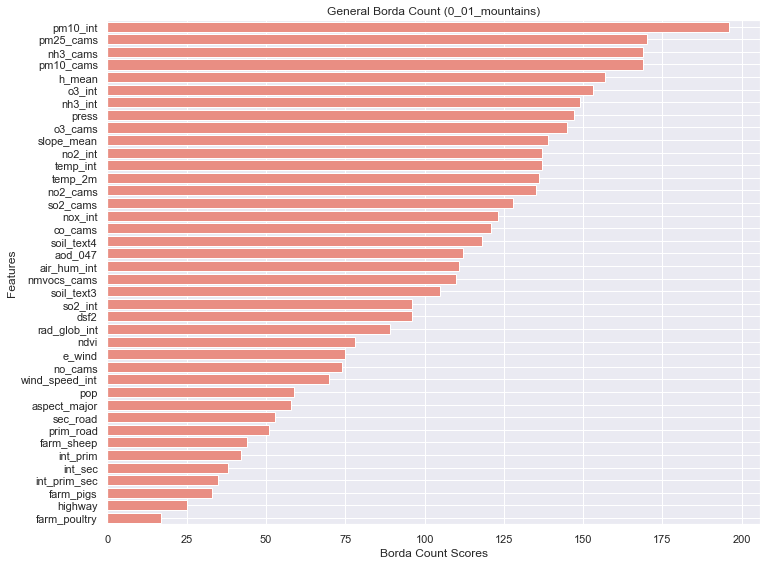
\includegraphics[scale =0.45]{images/tests/0_01_mountainspm25_st.png}\label{fig:a}}\\
\subfloat[Pearson index results in the  24-31 March and 18-25 April periods.]{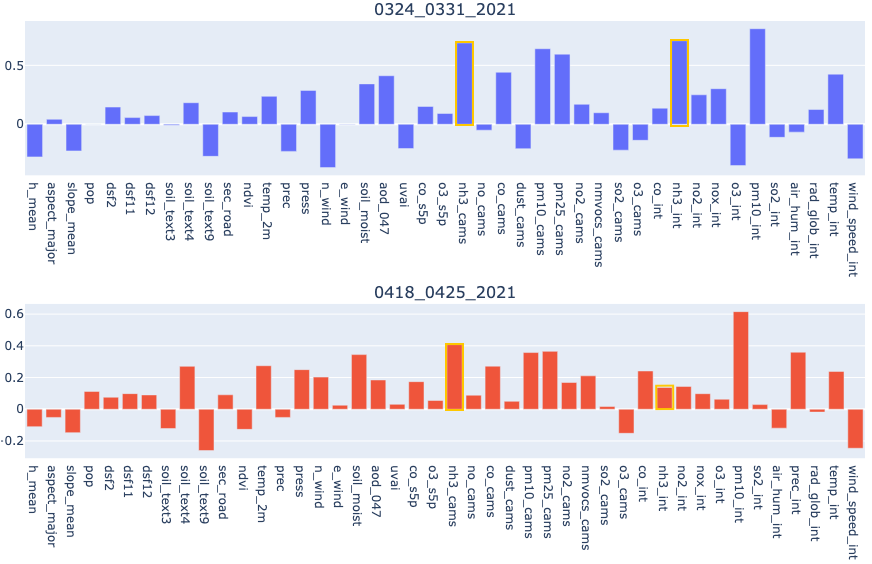
\includegraphics[scale =0.40]{images/tests/ammonia_effect_on_pm25_001mountains.png}\label{fig:b}}
\caption{Results obtained assuming PM2.5 as target variable with 10 Km resolution including mountains.}
\label{fig:fs_pm25}
\end{figure}
\subsection{NH3 as target variable}
Ammonia (NH3) is a reactive and soluble alkaline gas. It is one of the main sources of nitrogen pollution and comes from natural and anthropogenic sources, such as agriculture.\\
The process of ammonia evaporation commonly takes place when nitrogen is originated from the urea of animal livestock, and fertilize. \\
In the results obtained along the five periods, the ammonia provided by the CAMS model ('nh3\_cams') stands out, because it is strongly correlated, and represents the same pollutant as well.
We can observe in figure \ref{fig:fs_nh3} also variables related to PM10 and PM2.5 ('pm10\_int', 'pm10\_cams', 'pm25\_int' and 'pm25\_cams'), because ammonia contribute for the formation of secondary particulate matter \cite{dai2019concentrations} \cite{zhu2015sources}.\\
The correlation of ammonia in relation to intensive agriculture should be visible by the high positive correlation with agricultural areas (modelled by 'dsf2' variable), in particular used for maize cultivation ('siarl9') .\\
It is observable also the votes received by the variable that models the soil moisture, always with a positive correlation in relation to the target variable. This could be explained by the abundance of ammonia-oxidizing bacteria that increase with soil moisture \cite{avrahami2007response}.  \\
Other important weighted features are the ones related to intense farming ('farms' and 'farm\_pigs') which are responsible for ammonia release thanks to the chemical reaction of urea.\\
Animal urine and faeces imply the release of ammonia and methane in the atmosphere, respectively \cite{saggar2004review}.
So we can suggest that ammonia in Lombardy should be very related to the use of fertilizer in agricultural areas and animal livestock in farms.
\bigbreak
\pagebreak
\clearpage
\begin{figure}[H]
\centering
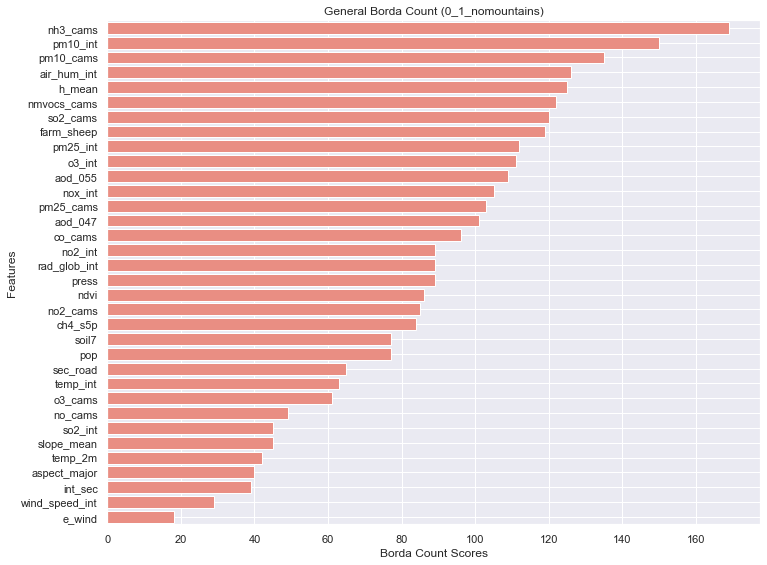
\includegraphics[scale =0.50]{images/tests/0_1_nomountainsnh3_st.png}
\caption{FS results obtained with Ammonia (NH3) as target variable with 1 Km resolution excluding mountains.}
\label{fig:fs_nh3}
\end{figure}
So overall, the results obtained in feature selection demonstrate two things.\\
First, fine particulate should be very correlated with ammonia in the manuring period (spring). Second, ammonia is strictly related to agriculture and farming activity, in accordance with previous studies.\pagebreak
\section{Data Modelling Results}
\label{sec:modelling2}
This section collected the interpretation of the ML models' results. 
\subsection{Interpretation of validation results with ARPA sensor}
The errors obtained in the results by the validation through particle matter decrease with higher resolution.\\
Higher resolution implies a larger number of samples for training and so a better accuracy as consequence.\\
With the PM2.5 target variable at 10 km resolution, there is a lower statistical accuracy than at 1km.
With 10 km resolution MAE reaches a maximum value of 1.448 ug/m\textsuperscript{3} (Tables \ref{tab:res10km}), while for 1 km resolution it does not exceed 0.347 ug/m\textsuperscript{3} (Tables \ref{tab:res1km})
\par 
With ammonia as the target variable the error is higher.
In relation to the results obtained by RF at 1 km with PM2.5 as target variables, the ones of ammonia has a MAE that has a maximum value of 0.939 ug/m\textsuperscript{3} in the September period (table \ref{tab:nh3RF})

\begin{table}[H]
\begin{tabular}{lrrrrr}
\toprule
  &  24/03-31/03 &  18/04-25/04 &  17/07-24/07 &  3/09-10/09 &  7/10-14/10 \\
\midrule
  MAE\_sensor ($\mu$g/m\textsuperscript{3}) &        1.448 &        1.093 &        0.646 &       0.898 &       0.841 \\
RMSE\_sensor ($\mu$g/m\textsuperscript{3}) &        1.940 &        1.362 &        0.868 &       1.165 &       1.080 \\
 MSE\_sensor ($\mu$g\textsuperscript{2}/m\textsuperscript{6}) &        3.772 &        1.874 &        0.776 &       1.376 &       1.197 \\
  R2\_sensor  &        0.872 &        0.766 &        0.683 &       0.870 &       0.793 \\
\bottomrule
\end{tabular}
\caption{Random Forest statistics for PM2.5 at 10 km, excluding zones with mountains.}
\label{tab:res10km}
\end{table}
\begin{table}[H]
\begin{tabular}{lrrrrr}
\toprule
  &  24/03-31/03 &  18/04-25/04 &  17/07-24/07 &  3/09-10/09 &  7/10-14/10 \\
\midrule
  MAE\_sensor ($\mu$g/m\textsuperscript{3}) &        0.347 &        0.234 &        0.156 &       0.199 &       0.146 \\
RMSE\_sensor ($\mu$g/m\textsuperscript{3}) &        0.624 &        0.392 &        0.261 &       0.327 &       0.232 \\
 MSE\_sensor ($\mu$g\textsuperscript{2}/m\textsuperscript{6}) &        0.411 &        0.158 &        0.069 &       0.113 &       0.054 \\
  R2\_sensor  &        0.990 &        0.985 &        0.982 &       0.993 &       0.991 \\
\bottomrule
\end{tabular}
\caption{Random Forest statistics for PM2.5 at 1 km, excluding zones with mountains.}
\label{tab:res1km}
\end{table}

\begin{table}[H]
\begin{tabular}{lrrrrr}
\toprule
  &  24/03-31/03 &  18/04-25/04 &  17/07-24/07 &  3/09-10/09 &  7/10-14/10 \\
\midrule
 MAE\_sensor ($\mu$g/m\textsuperscript{3}) &        0.483 &        0.280 &        0.526 &       0.939 &       0.386 \\
RMSE\_sensor ($\mu$g/m\textsuperscript{3}) &        0.993 &        0.558 &        1.184 &       2.316 &       0.860 \\
 MSE\_sensor ($\mu$g\textsuperscript{2}/m\textsuperscript{6}) &        1.199 &        0.430 &        1.556 &       6.147 &       1.121 \\
  R2\_sensor  &        0.997 &        0.992 &        0.994 &       0.987 &       0.990 \\
\bottomrule
\end{tabular}
\caption{Random Forest statistics for NH3 at 1 km, excluding zones with mountains.}
\label{tab:nh3RF}
\end{table}
\begin{table}[H]
\begin{tabular}{lrrrrr}
\toprule
  &  24/03-31/03 &  18/04-25/04 &  17/07-24/07 &  3/09-10/09 &  7/10-14/10 \\
\midrule
 MAE\_sensor ($\mu$g/m\textsuperscript{3})&        1.904 &        2.287 &        3.126 &       2.743 &       3.146 \\
RMSE\_sensor ($\mu$g/m\textsuperscript{3}) &        2.570 &        3.341 &        4.205 &       3.841 &       4.465 \\
 MSE\_sensor ($\mu$g\textsuperscript{2}/m\textsuperscript{6}) &        6.867 &       11.579 &       18.068 &      16.405 &      21.579 \\
  R2\_sensor &        0.984 &        0.800 &        0.927 &       0.965 &       0.852 \\
\bottomrule
\end{tabular}
\caption{Neural Network statistics for NH3 at 1 km, excluding zones with mountains.}
\label{tab:nh3NN}
\end{table}
This difference should be given by a different number of ground sensor measurements of each pollutant. The size of samples of particulate matter is larger than the one for ammonia.
In figure \ref{fig:comparison-sensors} are shown the observations at 10km resolution of each different target variable used in this case study. The number of observations used (green cells) depends strictly on the number of ground sensor measurements. \\
The legend shows whether the cell has an added value by KNN or not. By these images, we can observe how the number of samples passed from 28 to 173 for PM2.5 as target variable and from 8 to 69 for NH3.
\begin{figure}[H] 
    \centering
    \subfloat[PM2.5 as target variable.]{%
        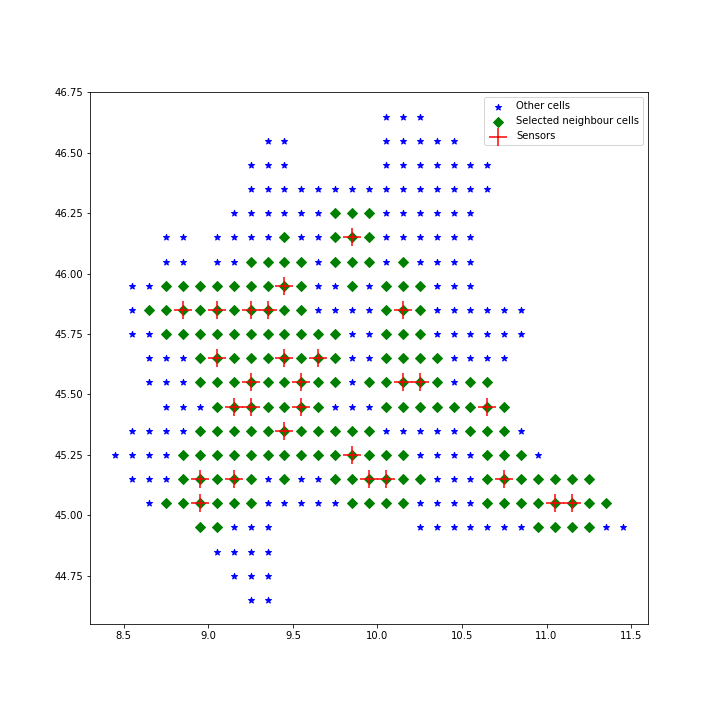
\includegraphics[width=0.5\textwidth]{images/pm25_sensors.png}%
        %
        }%
    \hfill%
    \subfloat[NH3 as target variable.]{%
        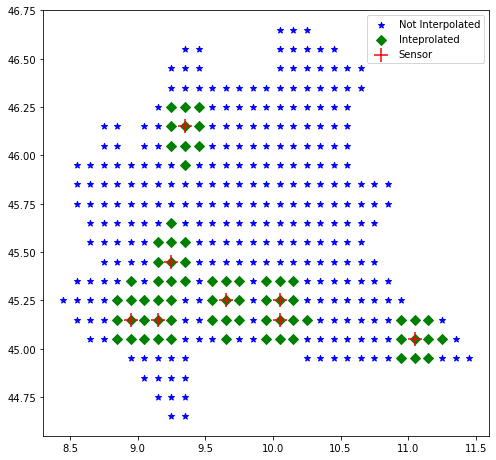
\includegraphics[width=0.5\textwidth]{images/nh3_sensors.png}%
        %
        }%
    \caption{These images show the spatial representation of the cells of the grid data obtained with the use of KNN with 10 km resolution.}
    \label{fig:comparison-sensors}
\end{figure}
We can observe also that generally, the Random Forest model makes more accurate predictions than the Neural Network by Keras (Tables \ref{tab:nh3RF} and \ref{tab:nh3NN}). \\
This may be because RF algorithm uses the ensemble learning method for regression, a technique that joins estimation from multiple models to have more accurate predictions than a single model.\\ 
R\textsuperscript{2} in each test assumes a positive value, meaning that the pollutants taken into consideration in this case study can be explained by the regression models. 
\pagebreak

\subsection{Importance of the FS}
The underlying tables provide model results if FS is before applied or not.

It can be observed that feature selection is meaningful for the pre-processing phase since aims at discarding eventually useless variables and taking only the ones relevant to the target variable. \\
In the results obtained, we can detect that selection of variable with FS assume a key role in reducing the training time resolutions (Tables \ref{fig:importance10km} and \ref{fig:importance1km}).\\
If the number of input variables is reduced the volume of data will decrease as the time needed to process them.\\
Instead, there is no visible difference in terms of accuracy in the results obtained in both.\\
These findings suggest that if a reduction of the input variables is applied the training will be faster without compromising its accuracy.
In conclusion, the difference between the results of this test and the ones run for each period show also the presence of overfitting in my models. Indeed, results obtained with temporal hold-out validation (in particular for  R\textsuperscript{2}) show how the \acrshort{rf} model can't make accurate predictions about new data (which comes from a different period).  

\begin{table}[H]
\centering
\subfloat[10 km resolution.]
{\begin{tabular}{lrr}
\toprule
 &  With FS & Without FS \\
  \midrule
 MAE\_sensor ($\mu$g/m\textsuperscript{3}) &        2.123  &        2.061 \\
RMSE\_sensor ($\mu$g/m\textsuperscript{3}) &        2.645 &        2.567 \\
 MSE\_sensor ($\mu$g\textsuperscript{2}/m\textsuperscript{6}) &        6.997  &       6.592 \\
  R2\_sensor  &        0.130  &         0.176\\
   Training time (s) & 2.402 & 3.637 \\
\end{tabular}
\label{fig:importance10km}}
\\
\subfloat[1 km resolution.]
{\begin{tabular}{lrr}
\toprule
& With FS &  Without FS\\
\midrule
 MAE\_sensor ($\mu$g/m\textsuperscript{3})&        2.677 &        2.660 \\
RMSE\_sensor ($\mu$g/m\textsuperscript{3})&        3.230  &        3.252\\
 MSE\_sensor ($\mu$g\textsuperscript{2}/m\textsuperscript{6})&        10.434 &        10.575  \\
  R2\_sensor &        -0.268 &        -0.285 \\
   Training time (s) & 17.298 & 24.338 \\
 \label{fig:importance1km}
\end{tabular}}
\caption{Random Forest statistics for PM2.5, including zones with mountains using or not FS.}
\end{table}